% !TEX root = jbsilvaThesis.tex

\chapter{\label{chp:pseudo}Pseudospinodal in Heterogenous Systems with Long-Range Interactions}

As previously described the spindodal is defined only in a \mf\ system where the   interactions are long-range. To study nucleation near the spinodal with impurities, the spinodal field must be measured for different percentages of impurities. The process of measuring the \ps\ in the pure system will now be motivated and described. 

\section{Determining the Pseudospinodal}
To measure the \ps\ the properties of the susceptibility $\chi$ in an Ising system near criticality will be used.   %%
%%
\begin{equation}
\label{eq:sus_spinodal}
\chi \propto \frac{1}{(h-h_s)^\frac{1}{2}}
\end{equation}%%
%%
The process of measuring the spinodal field is started by simulating the system for a sufficient time to assure equilibrium is reached before measuring the susceptibility. The susceptibility is measured for a system which is not undergoing a transition such as nucleation. This process is repeated for different values of $h$ and for many realizations of the system. A linear fit is performed using Eqn.~\eqref{eq:sus_spinodal} after taking a logarithm on both sides of the equation to obtain an estimate of the value of the spinodal field $h_s$.      %%
%%

\begin{figure}[!h]
    \centering
      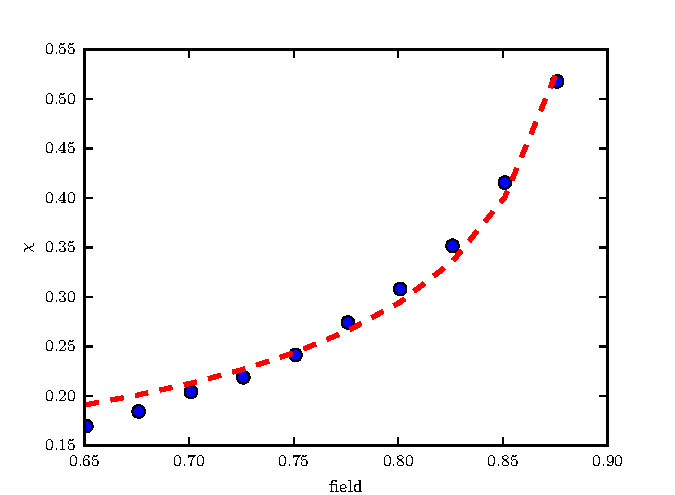
\includegraphics[scale=0.975]{Figures/spinodal/exampleSusFit1n.pdf}
    \caption{Example of the fit of the susceptibility to Eq.~\eqref{eq:sus_spinodal}  for a \het\ Ising system with $L=115$ and $\approx 3.75\%$ density of fixed spins in the stable direction with uniformly random chosen coordinates. The fitting parameters were $h_s$ and the prefactor of $\chi$. }
  \label{fig:ps_fit}
\end{figure}%%
%%

\section{The Pseudospinodal in Heterogeneous Ising Systems}

The behavior of the \ps\ in a diluted Ising system has been studied by Liu et al.~\cite{kangdilute} where it was shown that the dilution changes the value of the \ps\ field. In this section I will show that the effect of disorder in the form of fixed sites can be understood as imposing an effective field on the system in addition to the change of the value of $h_s$. The simulation will show that the assumptions in Eqn.~\eqref{eq:heter_w_field} are reasonable and confirmed by simulation. 
%%
\begin{figure}[!h]
  \centering
  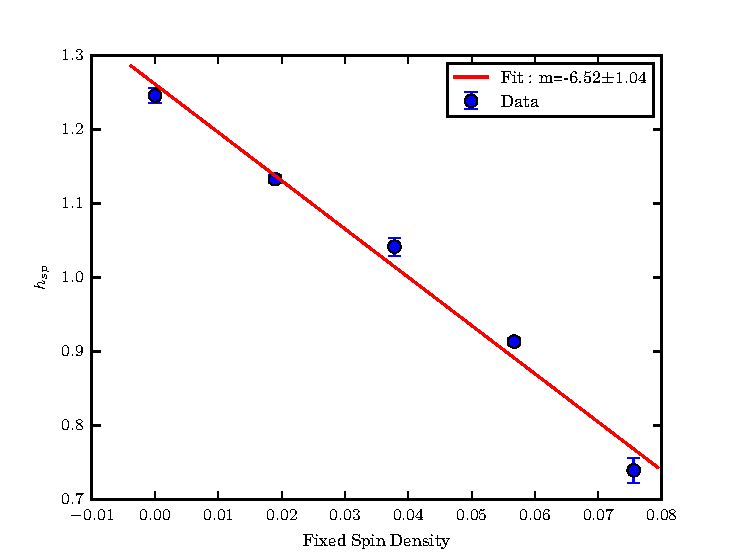
\includegraphics[scale=1.0]{Figures/spinodal/fixSpin1n_115.pdf}
  \caption{The value of $h_s$ for $L=115$ and fixed spins in the stable direction with an uniformly random choice of coordinates.}
  \label{fig:ps_heter_n}
\end{figure}%%
\begin{figure}[!h]
  \centering
      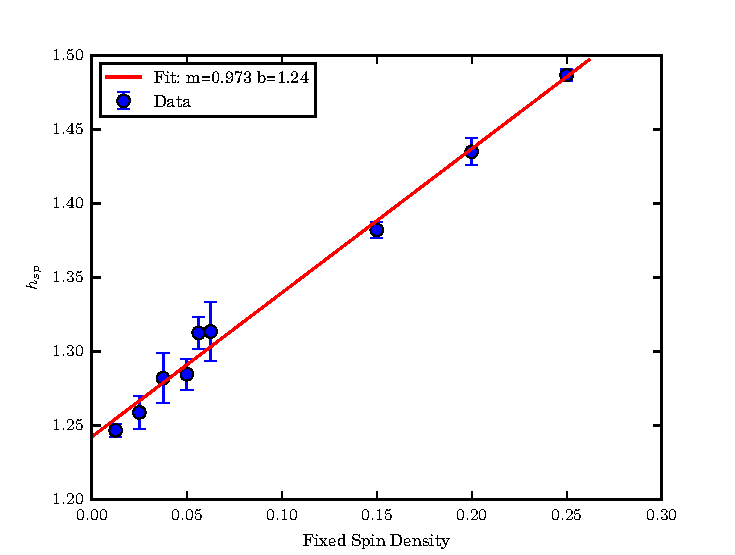
\includegraphics[scale=1.0]{Figures/spinodal/fixSpin1p_200.pdf}
  \caption{The value of $h_s$ for $L=115$ and fixed spins in the metastable direction with an uniformly random choice of coordinates.}
  \label{fig:ps_heter_p}
\end{figure}%%
%%

In Fig.~\ref{fig:ps_fit} the logarithm of the susceptibility is shown for a system with $3.75\%$ of fixed stable state spins distributed with a uniformly random choice of coordinates as well as the fit of Eqn.~\eqref{eq:sus_spinodal} used to obtain an estimate for the \ps\ field. The closer the approach to the \ps\ field, the greater the accuracy of the fit to Eqn.~\eqref{eq:sus_spinodal}. Hence the linear fits where performed with   the ten measurements closest to the spindodal field. As the \ps\ field is approached, the nucleation rate is increased, limiting how close the field in the Monte Carlo simulation can be to the spinodal field. Additionally if the nucleation rate is too high, the assumption that the system is not undergoing nucleation in measuring the susceptibility will be violated creating a difficulty in using Eqn.~\eqref{eq:sus_spinodal} to determine the \ps\ field. 

%%
%%
\begin{figure}[!h]
  \centering
      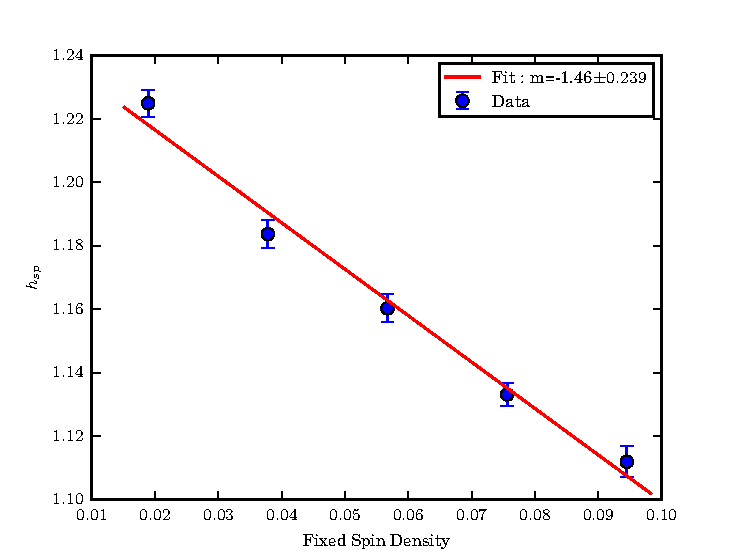
\includegraphics[scale=1.0]{Figures/spinodal/fixSpin0_115.pdf}
  \caption{The value of $h_s$ for  $L=115$ and a randomly distributed dilution of non-magnetic sites.}
  \label{fig:ps_heter_0}
\end{figure}%%
\begin{figure}[!h]
  \centering
      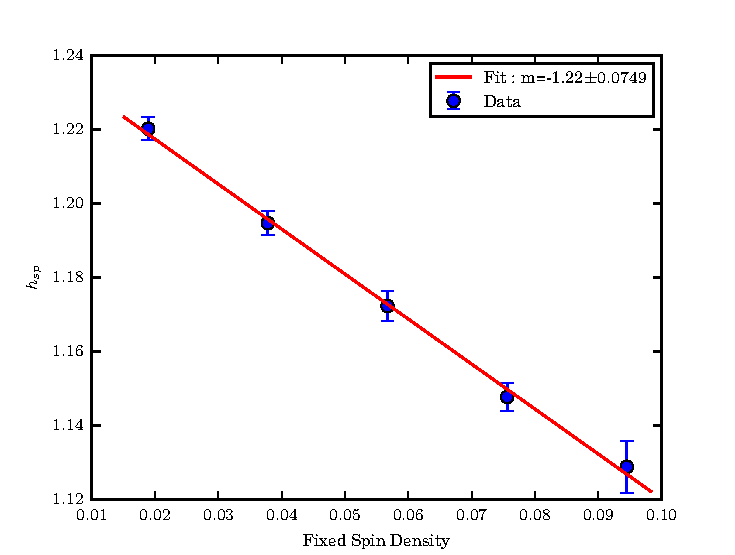
\includegraphics[scale=1.0]{Figures/spinodal/fixSpin1bQ_115.pdf}
  \caption{The value of $h_s$ for  $L=115$  and a quilt pattern distribution composed of an equal number of fixed spins in the stable and metastable directions. Figure~\ref{fig:ps_heter_0} and  Fig.~\ref{fig:ps_heter_pn} display similar slopes for their respective linear fits.}
  \label{fig:ps_heter_pn}
\end{figure}%%
%%

This process of measuring the \ps\ field was completed for multiple percentages of fixed stable spins. As discussed in Chapter~\ref{chp:nuc_details} the fixed spins behave similar to a random field along the direction of the fixed spins. This field increases as the number of fixed spins within an interaction range increases. Figure~\ref{fig:ps_heter_p} shows the predicted increase in the effective field as the percentage of \het\ sites is increased for fixed spins in the metastable direction. This behavior is explored further by changing the \het\ sites into stable spin fixed sites. In Fig.~\ref{fig:ps_heter_n} we observe the result of the susceptibility measurements for stable \het\ sites. Both results are consistent as expected from Eqn.~\eqref{eq:heter_w_field} of a slope given by the sum of the effective field and the spinodal field value for the pure Ising system. 

We would expect similar behavior for a diluted Ising system and a system with an equal amount \het\ sites chosen in the metastable and stable directions due to the  magnetic sites canceling each other in Eqn.~\eqref{eq:heter_w_field}. Hence only dilution effects remain. In Fig.~\ref{fig:ps_heter_pn} we observe the result of the susceptibility measurements for an equal mix of metastable and stable \het\ sites. As expected, we observe the predicted similarity of the behavior of these susceptibility results and the result of similar simulations in diluted systems in Fig.~\ref{fig:ps_heter_0}.    %%


Although the pseudospinodal for diluted systems is similar to the mixed metastable and stable \het\ system, the nucleation rates are not expected to be identical due to  fluctuations in the locations of the \het\ sites creating favorable locations for nucleation. This effect is expected to dominate as the percentage of \het\ sites is increased, and fluctuations of like spins nearing the critical droplet size become more likely.


To determine how the distribution of fixed spins  prevents a closer approach to the \ps, the minimum field difference between $h_s$  and $h$ was measured for varying amounts of fixed stable spins in a quilt pattern and fixed spin distribution of uniformly random chosen coordinates (see Fig.~\ref{fig:spinodalshift}). A metastable lifetime of at least $1000$ Monte Carlo steps was used as the criterion for the limiting value of $h$. 

As expected, an increase in this minimum field difference in Fig.~\ref{fig:spinodalshift}  is observed for the random disordered case relative to the quilt pattern due to the increase in the nucleation rate from the former case which lowers the nucleation barrier  at  localized sites. The \het\ nucleation effects of the  spatially uniform fixed spin case naturally increases the likelihood of the local pockets with a large amount of disorder become increasingly likely. 
%%
\begin{figure}[!h]
    \centering
      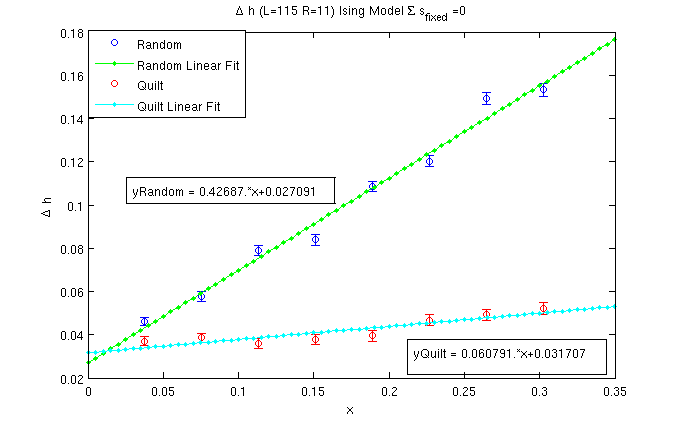
\includegraphics[scale=0.75]{Figures/spinodal/BalancedL115.png}
    \caption{The closest approach to the spinodal, $\Delta h$, as a function of the fixed spin density  in the stable direction with $L=115$. A spatially uniform distribution of fixed sites does not allow  $h_s$ to be approached as closely. }
  \label{fig:spinodalshift}
\end{figure}%%


The behavior of the \ps\ is now understood, which allows for the application of spinodal nucleation theory to the \het\ case. The application of percolation methods used in spinodal nucleation to \het\ nucleation will be focus of the following chapter. 
